\documentclass[a4paper,11pt]{report}
\usepackage[T1]{fontenc}
\usepackage[utf8]{inputenc}
\usepackage{lmodern}

\usepackage{verbatim}

\usepackage{hyperref}
\usepackage{graphicx}
\usepackage[english]{babel}

\usepackage{graphicx}
\usepackage{amsmath}

\usepackage{listings} % package for listing parts of code

\renewcommand*\footnoterule{}

\makeatletter
\renewcommand{\@chapapp}{}% Not necessary...
\newenvironment{chapquote}[2][2em]
  {\setlength{\@tempdima}{#1}%
   \def\chapquote@author{#2}%
   \parshape 1 \@tempdima \dimexpr\textwidth-2\@tempdima\relax%
   \itshape}
  {\par\normalfont\hfill--\ \chapquote@author\hspace*{\@tempdima}\par\bigskip}
\makeatother




% Book's title and subtitle
\title{\Huge \textbf{High Performance Computing with C++} \vspace{4mm} \\ \huge Final Report}
% Author
% \author{\textsc{First-name Last-name}\footnote{email address}}
\author{\textsc{Robert Schütze} \\ \vspace{3mm}\text{4140641}  \\
\vspace{3mm}\text{schuetze.r@web.de}}


\begin{document}

\makeatletter
    \begin{titlepage}
        \begin{center}
            
\includegraphics[width=0.5\linewidth]{logos/Uni_Logo-Grundversion_E1_A4_CMYK.eps}\\[4ex]
            {\huge \bfseries  \@title }\\[2ex] 
            {\LARGE  \@author}\\[30ex] 
            {\large \@date}
        \end{center}
    \end{titlepage}
\makeatother
\thispagestyle{empty}
\newpage



\tableofcontents
\newpage
\paragraph{Derivation of LJ-Force}\mbox{}\\
Suppose we have a list of N atoms with the position vectors $\vec{r}_k:=[x_k, y_k, z_k]^T$. The vector between a pair of atoms is defined as $\vec{r}_{ij}:=\vec{r}_j-\vec{r}_i$. The pair distance $r_{ij}$ is defined as the 2-norm of $\vec{r}_{ij}$:\\$r_{ij}:=\sqrt{(x_j-x_i)^2+(y_j-y_i)^2+(z_j-z_i)^2}$. The potential energy of an atom pair is given by (cite ???):
\begin{equation}
	E_{pot_{ij}} = 4\epsilon\left[\left(\dfrac{\sigma}{r_{ij}}\right)^{12}-
	\left(\dfrac{\sigma}{r_{ij}}\right)^{6}\right]\label{eq:Epotij}
\end{equation}
The parameters $\epsilon$ and $\sigma$ tune the potential strength and the resting distance respectively. To get the potential energy of the whole system, we have to sum over all atom pairs:
\begin{equation}
E_{pot}=\dfrac{1}{2}\sum_{ij,~i\neq j}E_{pot_{ij}}
\end{equation}
The force, which the i-th atom exerts on the k-th atom is the pair force:
\begin{equation}
\vec{f}_{ik}=\nabla_{\vec{r}_k} E_{pot_{ik}}=\dfrac{\partial E_{pot_{ik}}}{\partial r_{ik}}\cdot
\nabla_{\vec{r}_k}r_{ik} \label{eq:fik}
\end{equation}
Using Eq. \eqref{eq:Epotij}, the first part of Eq. \eqref{eq:fik} reads:
\begin{equation}
\dfrac{\partial E_{pot_{ik}}}{\partial r_{ik}} = \dfrac{24\epsilon (\sigma^6 r_{ik}^6-2\sigma^{12})}{r_{ik}^{13}}\label{eq:delEpotik}
\end{equation}
The first line of the gradient of the pair distance can be calculated as follows:
\begin{equation}
\dfrac{dr_{ik}}{dx_k}=\dfrac{1}{2r_{ik}}\cdot 2(x_k-x_i)\cdot (1-\delta_{ik}) \label{eq:drik}
\end{equation}
Applying the same principle from Eq. \eqref{eq:drik} to the other two coordinate axes and plugging it, togerther with the result from Eq. \eqref{eq:delEpotik}, into Eq. \eqref{eq:fik} yields:
\begin{equation}
\vec{f}_{ik}=\dfrac{24\epsilon (\sigma^6 r_{ik}^6-2\sigma^{12})}{r_{ik}^{14}}\cdot(1-\delta_{ik})\cdot\vec{r_{ik}}\label{eq:fikf}
\end{equation}












\begin{comment}

\chapter{Chapter 1}
This is an example of a citation \cite{timm2016lattice}. The corresponding paper can be found in the bibliography section at the end of this document.

Lorem ipsum dolor sit amet, consectetur adipiscing elit. Duis risus ante, auctor et pulvinar non, posuere ac lacus. Praesent egestas nisi id metus rhoncus ac lobortis sem hendrerit. Etiam et sapien eget lectus interdum posuere sit amet ac urna.

Example of normal equation
\begin{equation}\label{eq:LBE}
f_i(\mathbf{x}_j+\mathbf{c}_i\cdot\Delta t,t+\Delta t)=f_i(\mathbf{x}_j,t)
-\omega \left( f_i(\mathbf{x}_j,t)-f_i^\text{eq}(\mathbf{x}_j,t) \right)
\end{equation}

Example of aligned equation:
\begin{align}
  \rho(\mathbf{x}_j, t) &= \sum_i f_i(\mathbf{x}_j, t) \\
  \mathbf{u}(\mathbf{x}_j, t) &= \frac{1}{ \rho(\mathbf{x}_j, t)}
    \sum_i \mathbf{c}_i f_i(\mathbf{x}_j, t)
\end{align}

\section{section title}
Lorem ipsum dolor sit amet, consectetur adipiscing elit. Duis risus ante, auctor et pulvinar non, posuere ac lacus. Praesent egestas nisi id metus rhoncus ac lobortis sem hendrerit. Etiam et sapien eget lectus interdum posuere sit amet ac urna. Aliquam pellentesque imperdiet erat, eget consectetur felis malesuada quis. Pellentesque sollicitudin, odio sed dapibus eleifend, magna sem luctus turpis.

\begin{itemize}
  \item Example of a list
  \item Example of a list
  \item Example of a list
\end{itemize}

\chapter{Chapter 2}

\begin{figure}[h!]
  \begin{center}
   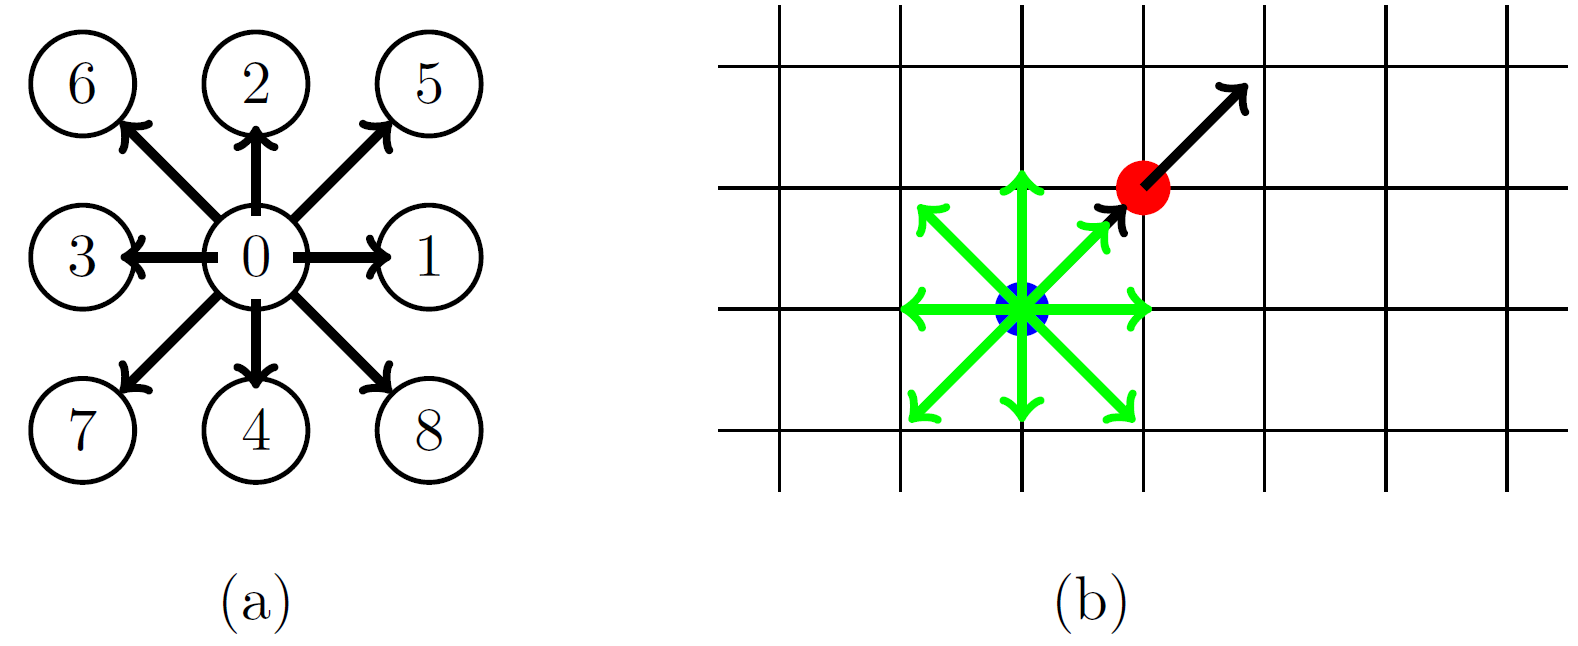
\includegraphics[width=10cm]{logos/Gitter_LBM.png}
   \caption{example figure}
  \label{fig:mesh}
  \end{center}
\end{figure}

\section{Section title}
Lorem ipsum dolor sit amet, consectetur adipisicing elit, sed do eiusmod tempor incididunt ut labore et dolore magna aliqua. Ut enim ad minim veniam, quis nostrud exercitation ullamco laboris nisi ut aliquip ex ea commodo consequat. \\ Duis aute irure dolor in reprehenderit in voluptate velit esse cillum dolore eu fugiat nulla pariatur. Excepteur sint occaecat cupidatat non proident, sunt in culpa qui officia deserunt mollit anim id est laborum.
id convallis magna eros nec metus. Sed vel ligula justo, sit amet vestibulum dolor. Sed vitae augue sit amet magna ullamcorper suscipit. Quisque dictum ipsum a sapien egestas facilisis.

\begin{table}[ht]
\caption{Sample table} % title of Table
\centering % used for centering table
\begin{tabular}{c c c c}
% centered columns (4 columns)
\hline\hline %inserts double horizontal lines
S. No. & Column\#1 & Column\#2 & Column\#3 \\ [0.5ex]
% inserts table
%heading
\hline % inserts single horizontal line
1 & 50 & 837 & 970 \\
2 & 47 & 877 & 230 \\
3 & 31 & 25 & 415 \\
4 & 35 & 144 & 2356 \\
5 & 45 & 300 & 556 \\ [1ex] % [1ex] adds vertical space
\hline %inserts single line
\end{tabular}
\label{table:nonlin} % is used to refer this table in the text
\end{table}

\section{Code listing}

here we provide a short example of code listing. For further information you can take look here:

\texttt{https://www.overleaf.com/learn/latex/code\_listing}

This is just meant to used if you think that there is some relevant part of code to be shown. Please do not append your whole implementation in the report.
\begin{lstlisting}[language=Python]
import numpy as np
    
def incmatrix(genl1,genl2):
    m = len(genl1)
    n = len(genl2)
    M = None #to become the incidence matrix
    VT = np.zeros((n*m,1), int)  #dummy variable

\end{lstlisting}

\newpage

Duis aute irure dolor in reprehenderit in voluptate velit esse cillum dolore eu fugiat nulla pariatur. Excepteur sint occaecat cupidatat non proident, sunt in culpa qui officia deserunt mollit anim id est laborum. \\ Lorem ipsum list:




\bibliographystyle{unsrt}
\bibliography{biblio}
\end{comment}

\end{document}
